	
	\subsection*{1.}
	
	On considère la fonction \(f\) définie par :
	\[
	f(x) = x^3 + 3x^2 - 9x - 1.
	\]
	
	\subsubsection*{a.}
	
	On a :
	\[
	f'(x) = 3x^2 + 6x - 9 = 3(x^2 + 2x - 3).
	\]
	
	\subsubsection*{b.}
	
	Le signe de \(f'(x)\) est celui du trinôme \(x^2 + 2x - 3\).
	
	Pour celui-ci :
	\[
	\Delta = 2^2 - 4 \times 1 \times (-3) = 4 + 12 = 16 = 4^2 > 0.
	\]
	
	Le trinôme a donc deux racines :
	\[
	x_1 = \dfrac{-2 + 4}{2} = 1 \quad \text{et} \quad x_2 = \dfrac{-2 - 4}{2} = -3.
	\]
	
	On sait que ce trinôme est positif sauf sur l'intervalle \(\left] -3 ; 1 \right[\) où il est négatif.
	
	Il en résulte que la fonction \(f\) est croissante sauf sur l'intervalle \(\left] -3 ; 1 \right[\) où elle est décroissante.
	
	Avec \(f(-3) = 26\) et \(f(1) = -6\), on a le tableau de variations :
	
	\begin{center}
	\begin{tikzpicture}[double distance=2pt]
		\tkzTabInit{$x$/1,$f'(x)$/1,$f(x)$/3}{$-\infty$,$-3$,$1$, $+\infty$}
		\tkzTabLine{,+,z,-,z, +}
		\tkzTabVar{-/,+/$26$,-/$-6$,+/}
	\end{tikzpicture}
\end{center} 

	
	\subsubsection*{c.}
	
	On sait qu'une équation réduite de la tangente à \(C_f\) au point d'abscisse \(-1\) est :
	\[
	y - f(-1) = f'(-1)(x - (-1)).
	\]
	
	Avec \(f(-1) = 10\) et \(f'(-1) = -12\), l'équation devient :
	\[
	y - 10 = -12(x + 1) \quad \Leftrightarrow \quad y = -12x - 12 + 10 \quad \Leftrightarrow \quad y = -12x - 2.
	\]
	
	\subsection*{2.}
	
	\subsubsection*{a.}
	
	La parabole a sa concavité tournée vers le haut : on a donc \(a > 0\) (on rappelle que \(a \neq 0\)).
	
	La parabole n'a pas de point commun avec l'axe des abscisses, donc le trinôme n'a pas de racines : \(\Delta < 0\).
	
	\subsubsection*{b.}
	
	Un point est commun si et seulement si ses coordonnées vérifient les équations des deux courbes ; il faut donc résoudre l'équation :
	\[
	x^3 + 3x^2 - 9x - 1 = 10x^2 + 8x + 8 \quad \text{ou} \quad x^3 - 7x^2 - 17x - 9 = 0.
	\]
	
	Ceci n'est pas possible, mais sur la figure, on voit que les deux courbes ont un point commun d'abscisse \(-1\) :
	\[
	f(-1) = 10 \quad \text{et} \quad g(-1) = 10 - 8 + 8 = 10.
	\]
	
	De plus, \(f'(-1) = -12\) et comme \(g'(x) = 20x + 8\), on a \(g'(-1) = -20 + 8 = -12\).
	
	Au point d'abscisse \(-1\), les deux fonctions ont le même nombre dérivé, donc la même tangente.
	
